\documentclass[a4paper,11pt,UTF8]{article}
\usepackage{ctex}
\usepackage{amsmath,amsthm,amssymb,amsfonts}
\usepackage{amsmath}
\usepackage[a4paper]{geometry}
\usepackage{graphicx}
\usepackage{microtype}
\usepackage{siunitx}
\usepackage{booktabs}
\usepackage[colorlinks=false, pdfborder={0 0 0}]{hyperref}
\usepackage{cleveref}
\usepackage{esint} 
\usepackage{graphicx}
\usepackage{ragged2e}
\usepackage{pifont}
\usepackage{extarrows}
\usepackage{float}
\usepackage{caption}
\usepackage{bm}
\usepackage{multirow}
\usepackage{subfigure}
\usepackage{titlesec}
\usepackage[mathscr]{eucal}
\captionsetup[figure]{name={Figure}}
\titleformat{\section}{\Large\bfseries}{Chapter \thesection}{1em}{}
\titleformat{\subsection}{\large\bfseries}{\thesubsection}{1em}{}
\titleformat{\subsubsection}{\normalsize\bfseries}{\thesubsubsection}{1em}{}
%opening
\title{Here Is All Your Need}
\author{谢悦晋\quad 提高2201班}

\date{\today}
\begin{document}
\maketitle
这里收集了复变函数考试的基本知识点,希望能够帮助大家,知识点很多,大家挑重点看就好
\tableofcontents\newpage
\section{复数与复变函数}
这一章的考点实际比较少,只能出一些小题.下面是个人认为比较重要的概念:
\begin{enumerate}
	\item 主辐角(辐角主值)
	对于给定复数$z\neq0$,设$\alpha$有满足:
	$$\alpha\in\mathrm{Arg}z,\alpha\in(-\pi,\pi]$$
	则$\alpha$为辐角主值,且有:
	$$\operatorname{Arg}z=\operatorname{arg}z+2k\pi,\quad k=0,\pm1,\pm2,\cdots\cdots.$$
	\item 三角表示和指数表示
	$$z=|z|e^{i\theta}=|z|(\cos\theta+i\sin\theta)$$
	\item De Moivre公式
	$$z^n=[r(\cos\theta+i\sin\theta)]^n=r^n(\cos n\theta+i\sin n\theta).$$
	\item 复数方根
	
	设$z$是给定的复数,$n$ 是正整数,求所有满足$w^n=z$ 的复数$w$,称为把复数$z$开$n$ 次方,记作 $w=\sqrt[n]{z}$或 $w=z^{1/n}.$ \textbf{复数$z$的$n$次方根一般是多值的},公式如下:(也可用复平面单位根分解)
	$$z=r\operatorname{e}^{i\theta}\Rightarrow w_k=\sqrt[n]{z}=\sqrt[n]{r}\operatorname{e}^{i(\frac\theta n+\frac{2k\pi}n)},(k=0,1,\cdots,n-1).$$
	\item 无穷大和无穷远点,复平面和扩充复平面
	\item 复变函数极限存在,连续$\Leftrightarrow$实部虚部极限存在,连续
\end{enumerate}
\section{解析函数}
这一章会考构造解析函数的大题,对于常见的初等解析函数也会考小题,知识点如下
\begin{enumerate}
	\item 导数与微分
	这部分与实值函数一致,不多赘述
	\item 解析与解析函数
	
	$f(z)$ 在 $z_0$ 解析 $\Leftrightarrow$ $f(z)$在 $U(z_0,\delta)$ 可导
	
	$f(z)$ 在区域 $D$ 内的每一点解析$\Leftrightarrow$ $f(z)$ 在 D 内解析,称 $f(z)$ 是 D 内的解析函数
	
	\textbf{点解析$\Rightarrow$点可导,区间解析$\Leftrightarrow$区间可导}
	\item 点可导的充要条件
	
	函数$w=f(z)=u(x,y)+iv(x,y)$在点 $z=x+iy$ 处可导
	$\Leftrightarrow$\\
	$u(x,y)$ 和$v(x,y)$ 在点$(x,y)$ 处可微, 且满足C-R方程:
	$$\frac{\partial u}{\partial x}=\frac{\partial v}{\partial y},\quad\frac{\partial u}{\partial y}=-\frac{\partial\nu}{\partial x}$$
	\item \textbf{区域解析的充要条件}
	
	函数$w=f(z)=u(x,y)+iv(x,y)$在区域$D$内解析\\
	$\Leftrightarrow$$u(x,y)$ 和 $\nu(x,y)$在区域 $D$ 内可微,且满足$C-R$方程。
	\item 解析函数的调和性
	
	若函数 $f(z)=u(x,y)+iv(x,y)$ 在区域$D$ 内解析, 则 $u(x,y),v(u,y)$ 在区域 $D$ 内满足Laplace方程:(调和函数定义)
	$$\frac{\partial^2u}{\partial x^2}+\frac{\partial^2u}{\partial y^2}=0,\frac{\partial^2v}{\partial x^2}+\frac{\partial^2v}{\partial y^2}=0$$
	
	共轭调和函数: $u(x,y)$ 及 $v(x,y)$ 均为区域 $D$ 内的调和函数, 且满足C-R方程:则称$v$是$u$的共轭调和函数。(不要弄反了)
	\item \textbf{构造调和函数}
	
	已知实部 $u$, 求虚部 $v $(或者已知虚部 $v$, 求实部 $u$ ),使 $f(z)=u(x,y)+iv(x,y)$ 解析,且满足指定的条件。
	
	解决方法:\textbf{必须首先检验$u,v$是否为调和函数},然后利用解析函数满足C-R方程的性质,根据偏积分或全微分法解决
	\item 常见初等函数及其公式
	\begin{itemize}
		\item \textbf{指数函数}
		
		对于复数 $z= x+ iy, $称$w= \mathbf{e} ^x( \cos y+ i\sin y) $ 为指数函数, 记为$w=\exp z$ 或$w={e}^{z}.$
		
		性质:单值,除无穷远点处处连续,处处解析,以2k$\pi i$为周期
		\item 对数函数
		
		满足方程 $\mathbf{e}^w=z$ 的函数 $w=f(z)$ 称为对数函数,记作 $w=\mathrm{Ln}z.$,计算公式:
		$$
			z=|z|{e}^{i\mathrm{Arg}z}=e^ue^{iv}\Rightarrow\begin{cases}
				u=\ln |z|\\
				v=\arg z+2k\pi i
			\end{cases}\Rightarrow=w=\mathrm{Ln}z=u+iv=\ln |z|+\arg z+2k\pi i
		$$
		主值:$w=\ln z= \ln |z|+\arg z$,分支:任意固定的一个k,即为分支
		\item 幂函数
		
		函数$w=z^\alpha$\textbf{规定}为 $z^\alpha=\mathrm{e}^{\alpha\mathrm{Ln}z}(\alpha$为复常数,$z\neq0)$ 称为复变量 $z$的幂函数。还\textbf{规定}: 当$a$为正实数,且 $z=0$ 时,$z^{\alpha}=0.$(\textbf{不要将这种“规定”方式反过来作用于指数函数})
		
		\item 三角函数
		$$\cos z=\frac12(\mathrm{e}^{iz}+\mathrm{e}^{-iz}),\sin z=\frac1{2i}(\mathrm{e}^{iz}-\mathrm{e}^{-iz})$$
		性质:周期性、可导性、奇偶性、零点、三角公式以及求导法则与实函数一致,\textbf{有界性不成立}
		\item 反三角函数
		如果$\cos w= z, $则称$w$为复变量$z$的反余弦函数记为$w=\mathrm{Arc\cos z}.$.计算方式如下:
		$$z=\cos w=\frac12(\mathrm{e}^{iw}+\mathrm{e}^{-iw})\Rightarrow(\mathrm{e}^{iw})^2-2z\mathrm{e}^{iw}+1=0,$$
		\item 双曲函数与反双曲函数(不做要求,了解即可)
	\end{itemize}	
\end{enumerate}
\section{复变函数的积分}
\begin{enumerate}
	\item 复积分的性质与计算
	
	比较重要的性质是这个:$$
	\left|\int_Cf(z)\mathrm{d}z\right|\leq\int_C|f(z)||\mathrm{d}z|=\int_C|f(z)|\mathrm{d}s\leq \max_{z\in c}|f(z)| L
	$$
	注意积分中值定理在复积分中并不成立
	
	复积分的计算:化为第二类曲线积分或定积分计算,后面还会使用计算原函数,柯西积分公式,导数公式以及留数计算
	
	一个重要的结论:$$I=\oint_{|z-z_0|=r}\frac{\mathrm{d}z}{(z-z_0)^n}=\begin{cases}
		2\pi i,\quad n=1 \\0, \quad n\neq1
	\end{cases}$$
	\item 柯西积分定理
	
	设函数$f(z)$在单连通域$D$内解析, $\Gamma$为$D$内的任意一条简单闭曲线, 则有$$\displaystyle\oint_{\Gamma}f(z)\mathrm{d}z=0$$
	
	闭路变形原理: $\partial_D=C_1+C_2^-$,$f(z)$在D内解析,则有:$$\displaystyle\oint_{C_1}f(z)\mathrm{d}z=\oint_{C_2}f(z)\mathrm{d}z=\oint_\Gamma f(z)\mathrm{d}z$$
	
	复合闭路原理:$\partial_D=C_0+C_1^-+C_2^-+...+C_n^-$, 函数$f(z)$在D内解析,在$\overline{D}=D+C$上连续,则有
	$$\oint_{\partial_D}f(z)\mathrm{d}z=0,\quad \oint_{C_0}f(z)\mathrm{d}z=\sum_{k=1}^{n}\oint_{C_k}f(z)\mathrm{d}z$$
	
	路径无关性:设函数 $f(z)$ 在单连通域 $D$ 内解析, $C_1,C_2$为$D$内的任意两条从$z_0$ 到$z_1$ 的简单曲线,则有
	$$
	\int_{C_1}f(z)\mathrm{d}z=\int_{C_2}f(z)\mathrm{d}z.
	$$
	
	原函数与Newton-Leibniz公式:与实函数相同
	\item 柯西积分公式
	
	如果函数 $f(z)$在简单闭曲线$C$所围成区域 $D$ 内解析, 在$\overline{D}=D+C$上连续,$z_0\in D$,则
	$$
	f(z_0)=\frac1{2\pi i}\oint_C\frac{f(z)}{z-z_0}\mathrm{d}z.
	$$
	应用:$
	\displaystyle\oint_C\frac{f(z)}{z-z_0}\mathrm{d}z=2\pi if(z_0).
	$
	\item 平均值公式
	
	如果函数 $f(z)$在 $|z-z_0|<R$ 内解析, 在$|z-z_0|\leq R$上连续,则有
	$$
	f(z_0)=\frac1{2\pi}\int_0^{2\pi}f(z_0+R\mathrm{e}^{i\theta})\mathrm{d}\theta.
	$$
	\item 最大模原理(压轴证明或许会考)
	
	如果函数 $f(z)$在$D$ 内解析,且不为常数,则在$D$内$\left|f(z)\right|$没有最大值。
	
	推论:
	\begin{itemize}
		\item 在区域$D$内解析的函数,如果其模在$D$内达到最大值, 则此函数必恒为常数。
		\item 若$f(z)$在有界区域$D$内解析,在$\overline{D}$上连续,则$|f(z)|$在D的边界上必能达到最大值。
	\end{itemize}
	\item 高阶导数公式
	
	如果函数 $f(z)$在区域 $D$ 内解析,在 $\overline{D}=D+C$ 上连续, 则 $f(z)$的各阶导数均在$D$ 上解析,且
	$$
	f^{(n)}(z)=\frac{n!}{2\pi i}\oint_C\frac{f(\zeta)}{\left(\zeta-z\right)^{n+1}}\mathrm{d}\zeta,\mathrm{~}(z\in D).
	$$
	\item 柯西不等式(压轴证明题或许会考)
	
	设函数$f(z)$在$|z-z_0|<R$内解析,且 $|f(z)|\leq M$,则
	$$
	|f^{(n)}(z_0)|\leq\frac{n!M}{R^n},\mathrm{~(n=1,2,\cdots)}.
	$$
	
	\item 刘维尔定理(压轴证明题或许会考)
	
	设函数$f(z)$在全平面上解析且有界,则$f(z)$为一常数
	
	
\end{enumerate}

\section{解析函数的级数表示}
这一章会考洛朗级数展开的大题, 不麻烦,一定要掌握
\begin{enumerate}
	\item 复数序列
	
	复数序列收敛$\Leftrightarrow$实部虚部收敛
	$\{|z_n|\}$收敛 $\Leftarrow$ $\{z_n\}$ 收敛,  $\lim_{n\to+\infty}|z_n|=0\Leftrightarrow\lim_{n\to+\infty} z_n=0.$
	\item 复数项级数
	
	复数项级数收敛$\Leftrightarrow$实部虚部级数收敛, 绝对收敛则级数收敛
	
	$\sum z_n\Leftarrow \lim_{n\to\infty}z_n=0$
	\item 复变函数项级数
	
	这一部分收敛域,和函数等的定义与实变函数项级数的定义基本相同
	\item \textbf{幂级数}
	\begin{itemize}
		\item Abel定理与收敛半径收敛圆
		\item 求幂级数半径的Cauthy-Hadamard定理
		\item 幂级数的运算性质以及分析性质基本和实变幂级数基本相同
	\end{itemize}
	\item \textbf{将函数展开为泰勒级数的方法}
	
	\textbf{展开请务必带上收敛域!展开请务必带上收敛域!展开请务必带上收敛域!}
	
	Taylor定理(理论依据):设函数 $f(z)$ 在区域 $D$ 内解析,$C=\partial D$,$z_0\in D$, $R=\min_{z\in C}
	|z-z_0|$,则当$|z-z_0|<R$时,有
	$$
	f(z)=\sum_{n=0}^{+\infty}a_n(z-z_0)^n,\quad a_n=\frac1{n!}f^{(n)}(z_0)=\frac1{2\pi i}\oint_l\frac{f(z)}{\left(z-z_0\right)^{n+1}}dz.
	$$
	对于给定的函数,收敛半径等于展开点到$f(z)$最近一个奇点$\tilde{z}$的距离, 以下是具体的计算方法
	\begin{itemize}
		\item 直接展开: 利用泰勒定理计算$a_n$,下面是几个常见的Taylor展开式:
		\begin{align*}
			{e}^{z}&=\sum_{n=0}^{+\infty}\frac{z^{n}}{n!}={1}+z+\frac{z^{2}}{2!}+\cdots+\frac{z^{n}}{n!}+\cdots,|z|<+\infty.\\
			\sin z &=\sum_{n=0}^{+\infty}(-1)^n\frac{z^{2n+1}}{(2n+1)!}=z-\frac{z^3}{3!}+\frac{z^5}{5!}-\cdots,|z|<+\infty. \\
			\cos z&=\sum_{n=0}^{+\infty}(-1)^n\frac{z^{2n}}{(2n)!}=1-\frac{z^2}{2!}+\frac{z^4}{4!}-\cdots,|z|<+\infty. \\
			\frac1{1-z}&=\sum_{n=0}^{+\infty}z^n=1+z+z^2+z^3\cdots, |z|<1
		\end{align*}
		\item 间接展开: 利用已知函数的展开式,通过有理运算、代换、\textbf{逐项求导积分}等方法展开,这一部分跟实变函数幂级数展开很像
	\end{itemize}
	\item \textbf{将函数展开为洛朗级数的方法}
	
	\textbf{展开请务必带上收敛域!展开请务必带上收敛域!展开请务必带上收敛域!}
	
	Laurent定理(理论依据): 设函数$f(z)$在圆环域$\quad D{:}R_1<|z-z_0|<R_2$ 内解析,则 $f(z)$ 一定能在此圆环域中展开为
	$$
	f(z)=\sum_{n=-\infty}^{+\infty}a_n(z-z_0)^n,a_n=\frac1{2\pi i}\oint_C\frac{f(\zeta)}{\left(\zeta-z_0\right)^{n+1}}\mathrm{d}\zeta(n=0,\pm1,\pm2,\ldots)
	$$
	$C$为在圆环域内绕 $z_0$ 的任何一条简单闭曲线。
	洛朗级数一般是将解析部分和和主要部分分开考虑,处理方法仍然和幂级数相同
	\begin{itemize}
		\item 直接展开法:根据洛朗定理直接计算展开系数,很麻烦,不考
		\item 间接展开: 利用已知函数的展开式,通过有理运算、代换、\textbf{逐项求导积分}等方法展开,这一部分跟实变函数幂级数展开很像
	\end{itemize}
	无论是直接展开法还是间接展开法,在求展开式之前,都需要根据函数的奇点位置,将复平面(或者题目指定的展开区域 )分为若干个解析环!
\end{enumerate}
\section{留数及其应用}
\begin{enumerate}
	\item 判断零点的阶数的方法
	\begin{itemize}
		\item 求在零点的导数,求到什么时候不为0为止,是几阶导数就是几阶零点
		\item 在零点展开为泰勒级数,改为如下形式:
		$$f(x)=(z-z_0)^m(a_m+a_{m+1}(z-z_0)+a_{m+2}(z-z_0)^2+...)$$
		$m$即为零点阶数
	\end{itemize}
	\item  奇点、孤立奇点、判断孤立奇点种类的方法
	
	首先明确奇点分为孤立奇点、非孤立奇点和支点(不管他,多值函数的一个概念),前两者尤其要区分开来,说不定会考这种东西
	
	奇点:不解析的点
	
	孤立奇点:在$z_0$某个去心邻域内处处解析的点
	
	非孤立奇点:在$z_0$任意去心邻域内都有不解析的点
	
	孤立奇点的分类(本质上是根据洛朗级数展开):
	\begin{itemize}
		\item 可去奇点:洛朗级数展开后无负幂次项
		$$\lim_{z\to z_0}f(z)=c$$
		\item $N$阶极点:洛朗级数展开后有$N$个幂次项, $N=1$ 称为简单奇点
		$$\lim_{z\to z_0}f(z)=\infty,f(z)=\frac{1}{(z-z_0)^N}(a_{-N}+a_{-N+1}(z-z_0)+...)$$
		\item 本性极点:洛朗级数展开后有无穷多个幂次项
		$$\lim_{z\to z_0}f(z)\text{不存在且不为}\infty$$
		
		注:求$\lim_{z\to z_0}f(z)$可以使用L'Hospital法则
	\end{itemize}
	下面给出了一些判断极点阶数的简便方法:
	\begin{itemize}
		\item 若 $f(z)=\dfrac{1}{(z-z_0)^N}\varphi(z)$, 其中$\varphi(z)$在 $z_{0}$点的邻域内解析且 $\varphi(z_0)\neq0$, 则$z_0$ 为$f(z)$的$N$阶极点
		\item 若$f(z){=}\dfrac{\varphi(z)}{\psi(z)}$,且 $z_0$为$\varphi(z)$的$m$阶零点,为$\psi(z)$的$n$阶零点,即 $f(z)=\dfrac{(z-z_0)^m\varphi_1(z)}{(z-z_0)^n\psi_1(z)}=\dfrac{(z-z_0)^m}{(z-z_0)^n}Q(z)$, 则$m\leq n$可去奇点,$m<n$为$(n-m)$阶奇点
	\end{itemize}
	注意:最最最本质的方法还是洛朗级数展开,这是最重要的
	\item 留数与留数的计算
	
	留数:在孤立奇点处的洛朗级数展开后$a_{-1}$的值
	$$\mathrm{Res}[f(z),z_0]=a_{-1}=\frac1{2\pi i}\oint_Cf(z)\mathrm{d}z,$$
	
	留数的计算方法:
	\begin{itemize}
		\item 可去奇点: $\mathrm{Res}[f(z),z_0]=0$
		\item 本性奇点:洛朗级数展开
		\item 极点:若为$m$阶极点,则计算公式如下
		$$\mathrm{Res}[f(z),z_0]=\frac{1}{(m-1)!}\lim_{z\to z_0}\frac{\mathrm{d}^{m-1}}{\mathrm{d}z^{m-1}}[(z-z_0)^mf(z)] $$
		特别的,如果是简单极点,如下:
		$$\mathrm{Res}[f(z),z_{0}]=\operatorname*{lim}_{z\to z_{0}}(z-z_{0})f(z)$$
	\end{itemize}
	\item 留数定理
	
	设 $f(z)$在区域 $D$ 内除有限个孤立奇点 $z_1,z_2,\cdots,z_n$ 外处处解析, $C$是$D $内包含各奇点的一条正向的简单闭曲线,则有:
	$$
	\oint_Cf(z)\mathrm{d}z=2\pi i\sum_{k=1}^n\operatorname{Res}[f(z),z_k].
	$$
	
	函数在无穷远点的性态:令$z=\dfrac1\xi$\,则点$z=\infty$ 对应于点$\xi=0$,相应地,$f(z)=f(\dfrac1\xi)\xlongequal{\Delta} \varphi ( \xi )$, 因此函数$f(z)$在无穷远点$z=\infty$的性态可由函数$\varphi(x)$在原点$\xi=0$的性态来刻画, 下面给出一个重要的公式
	
	设 $f(z)$在扩充平面上除有限个孤立奇点$z_1,z_2,\cdots,z_n,\infty$外处处解析,则$$\sum_{k=1}^n\operatorname{Res}[f(z),z_k]+\operatorname{Res}[f(z),\infty]=0,\quad\mathrm{Res}[f(z),\infty]=-\mathrm{Res}[f(\frac1{z})\frac1{z^2},0]$$
	如果一个区域内孤立奇点过多,或者阶数较高,可以考虑计算这个区域外的孤立奇点留数和
	\item 留数用于计算定积分
	\begin{itemize}
		\item 形如$\displaystyle\int_0^{2\pi}R(\cos\theta,\sin\theta)\mathrm{d}\theta$的积分
		
		要求:$R(u,v)$是 $u,v$的有理函数,即$R$是以$u,v$为变量的二元多项式函数或者分式函数
		
		方法:令$z=e^{i\theta}=\cos\theta+i\sin\theta, \mathrm{d}z=ie^{i\theta}\mathrm{d}\theta, \cos\theta=\dfrac{e^{i\theta}+e^{-i\theta}}2=\dfrac{z^2+1}{2z},\newline\sin\theta=\dfrac{z^2-1}{2iz}$, 则:
		$$\int_0^{2\pi}R(\cos\theta,\sin\theta)\mathrm{d}\theta=\oint_{|z|=1}R(\frac{z^2+1}{2z},\frac{z^2-1}{2iz})\frac1{iz}dz$$
		\item 形如$\displaystyle\int_{-\infty}^{+\infty}R(x)\mathrm{d}x$的积分
		
		要求:$R(x)=\frac{P(x)}{Q(x)}$其中$P(x),Q(x)$为多项式,分母多项式次数比分子至少高两次,分母无实数零点
		
		结论:
		$$
		\displaystyle\int_{-\infty}^{+\infty}R(x)\mathrm{d}x=2\pi i\sum_{k=1}^n\mathrm{Res}[R(z),z_k]
		$$
		其中$z_k$为上半平面的极点($k=1,2,\ldots,n$)
		\item 形如$\displaystyle\int_{-\infty}^{+\infty}R(x)e^{iax}\mathrm{d}x(a>0)$的积分
		
		要求:$R(x)=\dfrac{P(x)}{Q(x)}$其中$P(x),Q(x)$为多项式,分母多项式次数比分子至少高一次,分母无实数零点
		
		结论:
		$$
		\displaystyle\int_{-\infty}^{+\infty}R(x)e^{iax}\mathrm{d}x=2\pi i\sum_{k=1}^n\mathrm{Res}[R(z)e^{iaz},z_k]=A+iB
		$$
		其中$z_k$为上半平面的极点($k=1,2,\ldots,n$)
		
		特别地
		$$
		\int_{-\infty}^{+\infty}R(x)\cos ax\mathrm{d}x=A,\quad \int_{-\infty}^{+\infty}R(x)\sin ax\mathrm{d}x=B,
		$$
		\item 注:关于二三型中$R(z)$有实孤立奇点的情况,\textbf{考试不考}
		
		结论(围道积分法可以证明):
		$$
		\displaystyle\int_{-\infty}^{+\infty}R(x)\mathrm{d}x=2\pi i\sum_{k=1}^n\mathrm{Res}[R(z),z_k]+\pi  i\sum_{i=1}^n\mathrm{Res}[R(x),x_i]
		$$
		其中上半平面孤立奇点$z_k(k=1,2,...,n)$,实轴简单奇点$x_i(i=1,2,...,m)$
	\end{itemize}
	
	
\end{enumerate}
\section{共形映射}
这一章很难,我也没太学明白
\begin{enumerate}
	\item 伸缩率、旋转角和导数的几何意义
	
	设$f^\prime(z_0)\neq0$
	
	伸缩率:$\displaystyle\lim_{z\to z_0,\forall C}\frac{|w-w_0|}{|z-z_0|}=|f^\prime(z_0)|$
	
	衡量曲线经过映射后伸缩程度大小,$f^\prime(z_0)\neq0$时,伸缩率不变,这说明了任何一条经过$z_0$的曲线伸缩率不变
	
	旋转角:$\displaystyle\lim_{z\to z_0,\forall C}(\varphi - \theta)=\varphi_0-\theta_0=\arg f^\prime(z_0)$
	
	衡量曲线经过映射后旋转程度大小,$f^\prime(z_0)\neq0$时,旋转角不变,这说明了任何一条经过$z_0$的曲线旋转角不变
	
	保角性:两条曲线的交角大小和方向在映射前后保持不变(旋转角不变性可以得到)
	\item 第一类保角映射、第二类保角映射与共形映射
	
	第一类保角映射:满足保角性和伸缩率不变性的映射
	
	\textbf{判断方法}:$w=f(z)$在D内解析且导数恒不为0.则为第一类保角映射
	
	第二类保角映射:满足"保角性"(交角大小不变,方向相反)和伸缩率不变性的映射
	
	共形映射:满足保角性和伸缩率不变性的一一映射(双方单值)
	\item 给定区域D和映射$w=f(z)$,求像区域的方法
	
	理论保证:保域性定理、边界对应原理
	
	求解像区域的一般方法:
	
	一般来说, $w=f(z)$是在$D+\partial D$上的单射,设$w=u+iv,z=x+iy$,若$x,y$满足的是一般方程,我们需要将$x,y$用$u,v$表达出来,再将其带入$x,y$满足的方程中,若$x,y$满足的是参数方程,将$u,v$用$x,y$表达出来, 再带入$x,y$的参数方程,下面是具体步骤:
	\begin{itemize}	
		\item 首先将求点与像点之间的坐标变换关系

		令 $z=x+iy,w=u+iv$, 则有
		
		$\begin{cases}v=v(x,y)\\u=u(x,y),\end{cases}\Rightarrow\begin{cases}x=\boldsymbol{\varphi}(u,v),\\y=\boldsymbol{\psi}(u,v).&\end{cases}$ 
		
		\item 求边界曲线 $C$ 的象曲线 $\Gamma.$
		
		若$C$的方程为$\begin{cases}{x}={x}(t),\\{y}={y}(t),\end{cases}\Rightarrow\begin{cases}u=u(x(t),y(t)),\\v=v(x(t),y(t)),\end{cases}$
		
		若$C$的方程为$ F(x,y)=0,\Rightarrow F(\varphi(u,v),\psi(u,v))=0,$
		
		\item 求象区域
		
		方法1:沿边界 C 的正向找三点,考察象点的走向
		方法2:在区域 D 的内部找一点,考察象点的位置
	\end{itemize}
	\item 分式线性映射和几个初等函数构成的保形映射
	
	在介绍如何求此共形映射的方法之前,我们要先介绍处理其的主要工具:分式线性映射和几个初等函数构成的保形映射 
	
	\textbf{定义:}由分式线性函数
	$$
		w=\frac{az+b}{cz+d}(a,b,c,d\in C,\frac ac\neq\frac bd)
	$$
	构成的映射, 称为分式线性映射
	
	一般形式的分式线性映射可以由下面四种最简单的分式线性映射复合而成,并且分式线性映射在扩充复平面上是共形映射:
	\begin{itemize}
		\item 平移映射
		$$
		w=z+b,\quad(b\in C)\\
		$$
		他将点集沿着向量$\vec{b}$方向平移$|b|$,在扩充复平面上是共形映射
		
		\item 旋转映射
		$$
		w=\mathrm{e}^{i\theta_0}z,\quad(\theta_0\in C)
		$$
		它将点集旋转$\theta_0$,在扩充复平面上是共形映射
		
		\item 相似映射
		$$
		w=rz\quad(r>0)
		$$
		它将曲线相似的变化$r$倍,在扩充复平面上是共形映射
		
		\item 反演(倒数)映射
		$$
		w=\frac1z
		$$
		它将单位圆内(外)的点映射到单位圆外(内),且辐角反号,在扩充复平面上是共形映射
	\end{itemize}
	关于反演映射,他是由两个特殊的对称映射构成的:
	\begin{itemize}
		\item 关于单位圆周的对称映射:$$w=\frac1{\overline{z}}$$(对称点到圆心距离之积为$R^2$)
		\item 关于实轴的对称映射:$$w=\overline{z}$$
	\end{itemize}
	倒数映射和平移旋转映射都具有保圆性,因此分式线性映射也是具有保圆性的,约定将直线看作半径无穷大的圆,则分式线性映射能在扩充复平面上将圆映射成圆,并且有\textbf{以下结论成立:}
	\begin{itemize}
		\item 给定圆上没有点映射成无穷远点,则映射为半径有限的圆
		\item \textbf{给定圆有一点映射成无穷远点,则被映射成直线}
		\item \textbf{对于给定的圆弧(或直线段),若其中一端点映射成无穷远点,则被映射成射线}
	\end{itemize}
	
		分式线性映射求圆像曲线的方法:
	\begin{itemize}
		\item 分解为四种简单映射的复合
		\item 利用保圆性,选定三点定圆
		\item  综合利用保圆性与保角性: 找出原像曲线中的一些特殊点的像点, 找出特殊曲线(坐标轴)的像,利用原像之间的夹角等关系确定像的关系
	\end{itemize}
	
	分式线性映射的保对称点性:$z_1,z_2$关于$C$对称,则在分式线性映射,它们的象点$w_1,w_2$ 关于像圆$C^\prime$对称
	
	唯一决定分式线性映射的条件(对应点公式):
	
	在$z$平面上任给三个不同的点$z_1,z_2,z_3,$在$w$平面上也任给三个不同的点$w_1,w_2,w_3$,则存在唯一的分式线性映射,把$z_1,z_2,z_3$分别依次地映射为$w_1,w_2,w_3$,且满足:
	$$
	\frac{w-w_1}{w-w_2}:\frac{w_3-w_1}{w_3-w_2}=\frac{z-z_1}{z-z_2}:\frac{z_3-z_1}{z_3-z_2}.
	$$
	推论:
	\begin{itemize}
		\item 若$z_k$或$w_k$ 中有一个为$\infty$,则只须将对应点公式中含有$\infty$的项换为1
		\item  设$w=f(z)$是一分式线性映射,且有$f(z_1)=w_1$以及$f(z_2)=w_2$,则它可表示为
		$$
		\frac{w-w_1}{w-w_2}=k\frac{z-z_1}{z-z_2}\quad(k\text{为复常数)}
		$$
		特别地,当$w_1=0,w_2=\infty$时,有:
		$$
		w=k\frac{z-z_1}{z-z_2}\quad(k\text{为复常数})
		$$
	\end{itemize}
	幂函数$w=z^n,n\geq2$
	
	特点:$|w|=r^n,\arg w=n\theta,n\theta<2\pi$, 扩大顶点在原点的角形域
	
	保形性:解析性,$z$平面不是双方单值
	
	结论:除原点外为第一类保角映射,对z加以控制可以变成共形映射
	
	指数函数$w=e^z$
	
	特点:指数函数讲水平带形区域变为角形域
	
	保形性:解析性,$z$平面不是双方单值的
	
	结论:指数函数$w=e^z$在$z$平面上是第一类保角映射
	
	注:水平带形域$0<y<h<2\pi$,此时指数函数为一一映射,故为共形映射
	
	\begin{figure}[H]
		\centering
		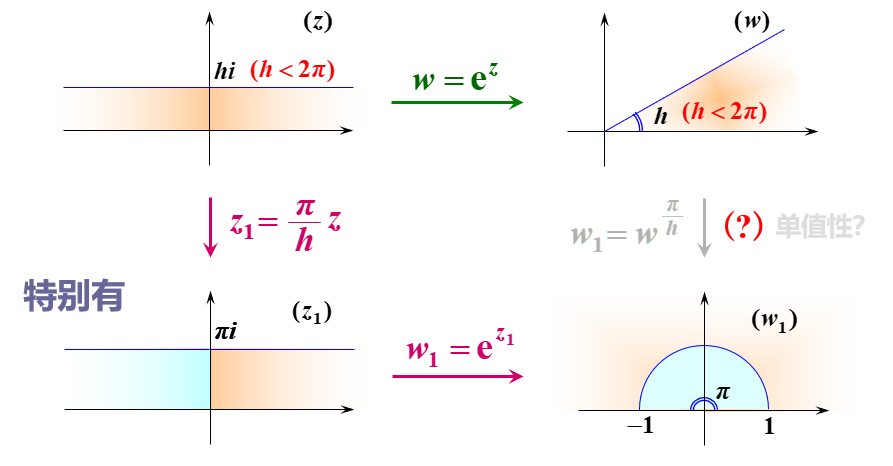
\includegraphics[width=0.7\textwidth]{6.1.png}
	\end{figure}
	
	
	\item 给定原像区域D和像区域G,求共形映射$w=f(z)$的方法(基本问题)	
	
	理论保证:黎曼存在唯一性定理
	
	主要步骤:
	\begin{itemize}
		\item 预处理
		
		使用简单的分式线性映射、幂函数、指数函数将边界变为至多两段圆弧构成
		\item 将区域映射成角形域/带形域
		
		将区域边界的一个交点$z_1$映射为$\infty$(使用$w=k\dfrac1{z-z_1}$or $w=k\dfrac{z-z_2}{z-z_1}$)
		
		\item  将角形域/带形域映射为上半平面
		
		使用$w=z^n,w=\sqrt[n]z,w=e^n$
		\item 将上半平面映射为单位圆域
		
		使用$w=\dfrac{z-i}{z+i},w=e^{i\theta_0}\dfrac{z-z_0}{z-\overline{z}_0}$
	\end{itemize}

\end{enumerate}
\section{傅里叶变换}
\begin{enumerate}
	\item 定义	
	傅里叶正变换
	$$
	F(w)=\int_{-\infty}^{+\infty}f(t)e^{-jwt}\mathrm{d}t=\mathcal{F}[f(t)]
	$$
	
	傅里叶逆变换
	$$
	f(t)=\frac1{2\pi}\int_{-\infty}^{+\infty}F(w)e^{jwt}\mathrm{d}t=\mathcal{F}^{-1}[F(w)]
	$$
	\item 单位冲激函数
	
	性质
	\begin{itemize}
	\item 筛选性质
	
	函数$f(t)$在$R$上有界且在$t=0$处连续:
	$$
	\int_{-\infty}^{+\infty}\delta(t)f(t)\mathrm{d}t=f(0)
	$$
	
	\item 对称性质
	$$\delta(t)=\delta(-t)$$ 
		\end{itemize}
	单位冲激的傅里叶变换
	\begin{itemize}
		\item 利用筛选性质:
		$$
			\mathcal{F}[\delta(t)]=\int_{-\infty}^{+\infty}\delta(t)e^{-jwt}\mathrm{d}t=\left.e^{-jwt}\right|_{t=0}=1
		$$
		\item 按照傅里叶逆变换:
		$$
		\mathcal{F}^{-1}[1]=\frac1{2\pi}\int_{-\infty}^{+\infty}1\cdot e^{jwt}\mathrm{d}w=\delta(t)
		$$
		\item 重要公式:
		$$
		\int_{-\infty}^{+\infty}e^{jwt}\mathrm{d}t=2\pi\delta(t)\
	$$
	\end{itemize}
	\item 傅里叶变换的性质
	\begin{itemize}
		\item 线性性质
		$$
		{\mathcal F}\left[af(t)+bg(t)\right]=aF(\omega)+bG(\omega).
		$$
		
		\item 位移性质
		$$
		\begin{aligned}&(1)\mathrm{~}\mathcal{F}[f(t-t_0)]=\mathrm{e}^{-j\omega t_0}F(\omega);\\&(2)\mathrm{~}\mathcal{F}^{-1}[F(\omega-\omega_0)]=\mathrm{e}^{j\omega_0t}f(t).\end{aligned}
		$$
		
		\item 相似性质
		
		设$a$为非零常数,则
		$$
		\mathcal{F}[f(at)]=\frac1{|a|}F{\left(\frac\omega a\right)}.
		$$
		若信号被压缩($a>1$),则其频谱被扩展
		
		若信号被扩展($a<1$),则其频谱被压缩
		
		\item 微分性质
		
		若$\lim_{|t|\to\infty}f(t)=0$,则
		$$
		\mathcal{F}[f^\prime(t)]=jwF(w)
		$$
		一般地, 若$\lim_{|t|\to\infty}f^{(k)}(t)=0,k=0,1,...,n-1$
		$$
		\mathcal{F}[f^{(n)}(t)]=(jw)^nF(w)
		$$
		同理,可以得到像函数的导数公式
		$$
		\begin{aligned}
			&\mathcal{F}^{-1}[F^\prime(w)]=-jtf(t)\\
			&\mathcal{F}^{-1}[F^{(n)}(w)]=(-jt)^nf(t)
		\end{aligned}
		$$
		
		\item 积分性质
		
		若$\lim_{t\to+\infty}\int_{-\infty}^tf(t)\mathrm{d}t=0$,则:
		$$
		\mathcal{F}[\int_{-\infty}^tf(t)\mathrm{d}t]=\frac1{jw}F(w)
		$$
		$\int_{-\infty}^tf(t)\mathrm{d}t\leftrightarrow\frac{F(w)}{jw}+\pi F(0)\delta(t)$
		
		\item Parseval等式
		$$
		\int_{-\infty}^{+\infty}f^2(t)\mathrm{d}t=\frac1{2\pi}\int_{-\infty}^{+\infty}|F(w)|^2\mathrm{d}w
		$$
	\end{itemize}
	\item 卷积和卷积定理
	
	设函数 $f_1(t)$ 与 $f_2(t)$在区间 $(-\infty,+\infty)$上有定义,如果广义积分$\int _{- \infty}^{+ \infty}f_1( \tau) f_2( t- \tau)d\tau$对任何实数$t$ 都收敛,则它在 $(-\infty,+\infty)$ 上定义了一个自变量为$t$ 的函数,称此函数为$f_1(t)$与$f_2(t)$的卷积,记为$f_1(t)*f_2(t)$,即
	$$
	f_1(t)*f_2(t)=\int_{-\infty}^{+\infty}f_1(\tau)f_2(t-\tau)\operatorname{d}\tau.
	$$
	性质:交换律、结合律、分配律
	
	卷积定理:
	
	设 $\mathcal{F}[f_1(t)]{=}F_1(\omega),\quad\mathcal{F}[f_2(t)]{=}F_2(\omega),\quad $则有:
	$$
	\begin{aligned}
		&\mathcal{F}[f_1(t)*f_2(t)]=F_1(\omega)\cdotp F_2(\omega);\\
		&\mathcal{F}^{-1}[F_1(\omega)*F_2(\omega)]=2\pi f_1(t)\cdotp f_2(t).
	\end{aligned}
	$$
	
\end{enumerate}
\section{拉普拉斯变换}
\begin{enumerate}
	\item 定义
	
	设函数 $f(t)$ 是定义在 $(0,+\infty)$上的实值函数,如果对于复参数$s=\beta+j\omega$,积分$F( s) = \int _0^{+ \infty}f( t) e^{- st}$d$t$ 在复平面$s$ 的某一区域内收敛,则称$F(s)$为$f(t)$ 的 Laplace 变换或像函数,记为$F(s)=\mathcal{L}[f(t)]$,即
	$$
	F(s)=\mathcal{L}[f(t)]=\int_{0}^{+\infty}f(t)e^{-st}\mathrm{d}t
	$$
	相应地,称 $f(t)$为$F(s)$的 Laplace 逆变换或像原函数
	$$
	f(t)=\mathcal{L}^{-1}[F(s)].
	$$
	
	存在性定理:设函数 $f(t)$ 当 $t\geq0$ 时,满足:
	\begin{itemize}
		\item 在任何有限区间上分段连续; 
		
		\item 具有有限的增长性,即存在常数$c$ 及$M>0$,使得$|f(t)|\leq M{e}^{ct}$,(其中,$c$ 称为函数 $f(t)$ 的“增长”指数)。
	\end{itemize}
	则象函数$F(s)$在半平面$\mathrm{Re} s>c$上一定存在且解析。
	
	注意:像函数$F(s)$的存在域一般是一个右半平面 Res$>c$,即只要复数 s 的实部足够大就可以了;在 Laplace 变换中的函数一般均约定在 $t<0$ 时为零,即函数$f(t)$等价于函数$f(t){u}(t)$
	
	常用函数的Laplace变换(重要)
	\begin{itemize}
		\item $\mathcal{L}[1]=\mathcal{L}[{\mathrm{sgn}(t)}]=\dfrac1s$
		\item $\mathcal{L}[\delta(t)]=1$
		\item $\mathcal{L}[t^m]=\dfrac{m!}{s^{m+1}}$
		\item $\mathcal{L}[e^{at}]=\dfrac1{s-a}$
		\item $\mathcal{L}[\cos at]=\dfrac{s}{s^2+a^2}$
		\item $\mathcal{L}[\sin at]=\dfrac{a}{s^2+a^2}$ 
	\end{itemize}
	\item Laplace变换的性质
	\begin{itemize}
		\item 线性性质和相似性质
		
		线性性质不用说
		
		相似性质:$\mathcal{L}[f(at)]=\frac1aF(\frac{s}{a}),a>0$
		
		\item 延迟性质和位移性质
		$$
		\mathcal{L}[f(t-\tau)]=e^{-s\tau}F(s),\tau\geq0
		$$
		位移性质:$\mathcal{L}[e^{at}f(t)]=F(s-a)$
		
		\item 微分性质
		$$
		\mathcal{L}[f^\prime(t)]=sF(s)-f(0)
		$$
		一般地:
		$$
		\mathcal{L}[f^{(n)}(t)]=s^nF(s)-\sum_{i=0}^{n-1}s^{n-1-i}f^{(i)}(0)
		$$
		像函数地的导数:
		$$
		F^{(n)}(s)=(-1)^n\mathcal{L}[t^nf(t)]
		$$
		
		\item 积分性质
		$$
		\mathcal{L}[\int_{0}^tf(t)\mathrm{d}t]=\frac1sF(s),\int_{0}^sF(s)\mathrm{d}s=\mathcal{L}[\frac{f(t)}{t}]
		$$
	\end{itemize}
	\item 卷积与卷积定理
	
	卷积:$\displaystyle f_1(t)*f_2(t)=\int_0^tf_1(\tau)f_2(t-\tau)\mathrm{d}\tau$
	
	卷积定理:
	
	设 $\mathcal{L}[f_1(t)]{=}F_1(\omega),\quad\mathcal{L}[f_2(t)]{=}F_2(\omega),\quad $则有:
	$$
	\begin{aligned}
		&\mathcal{L}[f_1(t)*f_2(t)]=F_1(s)\cdotp F_2(s);\\
		&\mathcal{L}^{-1}[F_1(s)*F_2(s)]=2\pi f_1(t)\cdotp f_2(t).
	\end{aligned}
	$$
	\item Laplace逆变换
	反演积分公式—Laplace逆变换公式
	$$
	f(t)=\frac1{2\pi j}\int_{\beta-j\infty}^{\beta+j\infty}F(s)e^{st}\mathrm{d}s
	$$
	
	求Laplace逆变换的方法
	\begin{itemize}
		\item 留数法
		$$
		f(t)=\sum_{k=1}^n\mathrm{Res}[F(s)e^{st},s_k],s_k\in\{s|\mathrm{Res}<c\}
		$$

		\item 查表法(重要,需要记住)
	\end{itemize}
	\item Laplace变换解常微分方程(组)
	
	工具: $\mathscr{L}[f^{(n)}(t)]=s^nF(s)-s^{n-1}f(0)-s^{n-2}f^{\prime}(0)-\cdots-f^{(n-1)}(0).$
	
	步骤:
	\begin{itemize}
		\item 将微分方程(组)化为象函数的代数方程(组);
		\item 求解代数方程得到象函数;
		\item 求 Laplace 逆变换得到微分方程(组)的解。
		
	\end{itemize}
\end{enumerate}
\end{document}    